\section{Evaluating Information Audits}
\label{sec:experiments}

We evaluate the surviving fraction under prospective nuisance interventions, inverse-information tails in synthetic experiments, and predictive projected Fisher in held-out discovery.

\subsection{Prospective Diagnosis Under a Nuisance Intervention}
\label{sec:prospective-diagnosis}

On Waterbirds \citep{sagawa2019distributionally}, the four groups cross bird class with background type and are written \emph{class/background}. We fully fine-tune ImageNet-initialized MobileNetV3-small models \citep{howard2019searching} with empirical risk minimization. Validation data fit the temperature and cross-fitted background probe. Eligible slices have accuracy at least the overall validation accuracy and negative log-likelihood at most the median across slices. Among them, we select the smallest surviving fraction, $\lambda_{\min}(\widehat F_g^{\rid})/\widehat J_{TT,g}$. After pilot experiments, this rule is fixed for five additional training seeds, 22--26. Each checkpoint, temperature, probe, selected slice, and audit constant is frozen before intervention scoring.

The rule selects \textbf{waterbird/water in all five seeds}: its validation surviving fraction is $24.8\%$, compared with $59.0\%$ for landbird/land, the other eligible slice. Held-out interventions recompose birds onto same-type or opposite-type backgrounds using the same extracted foreground layer, matte, and task labels. Same-type recomposition controls for the image-construction procedure. Selected-slice accuracy is $92.0\%$ on original images, $93.2\%$ under the control, and $40.6\%$ under opposite-type replacement: a \textbf{$52.6\pm1.4$ percentage-point controlled drop}, with a nominal 95\% normal-approximation interval across seeds.

Within the eligible set, minimum surviving fraction, minimum validation accuracy, and maximum validation NLL select waterbird/water in all five seeds, with a $52.6$-point controlled accuracy drop (Figure~\ref{fig:prospective-main}). Minimum raw and absolute projected information select landbird/land, with a $26.7$-point drop. Centering switches selection in all five seeds, identifying slice means as a ranking contributor; predictive Fisher retains waterbird/water in all five. Appendix~\ref{app:prospective-intervention} reports matched selectors, matrix and aggregation comparisons, and individual flip prediction.

\begin{figure}[t]
\centering
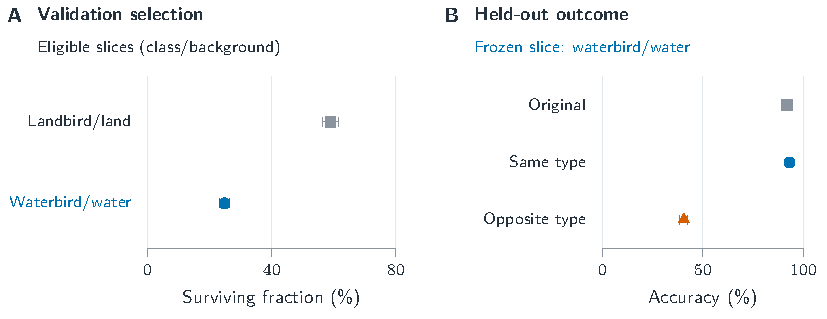
\includegraphics[width=\linewidth]{figures/fig03_prospective_main.pdf}
\caption[Validation selection anticipates held-out background sensitivity]{\textbf{A 52.6-point controlled accuracy drop in the selected group.}
(A) The uncentered feature--Schur fraction selects waterbird/water from two eligible groups; matched accuracy and NLL selectors agree. (B) Accuracy falls from 93.2\% under same-type background recomposition to 40.6\% under opposite-type recomposition, with bird foregrounds and labels preserved. Points show means and bars nominal 95\% normal-approximation intervals across five training seeds.
}
\label{fig:prospective-main}
\end{figure}

\subsection{Synthetic Classification and Tail Checks}
\label{sec:synthetic-validation}

Draw independent $s,r\sim N(0,1)$, set $z=s+\delta_e r$ and $Y=\mathbf1\{z>0\}$, and evaluate the nuisance-only logit $4s$. Environments use $\delta_e=0.35U_e^{1/\gamma}$, $U_e\sim\mathrm{Uniform}(0,1)$, with $\gamma=1$ in the main experiment. Five-seed mean accuracy is $94.54\%$ and $\CVaR_{0.95}$ of environment-mean NLL is $0.262$. Yet $I^{\FG}_{0.95}=(1.22\pm0.53)\times10^{-8}$ with $\varepsilon=10^{-12}$, despite raw information bounded below by one.

The inverse-information exponent is $0.498\pm0.003$, matching $\beta=\gamma/2=0.5$ in the geometric tail law of Theorem~\ref{thm:inverse-information-geometry} (Figure~\ref{fig:geometry-tails}). Log-survival regression uses the largest $5\%$ of inverse-information observations. Independent-branch experiments check the scalar portfolio law $\beta=K/2$ (Appendix~\ref{app:theory-tails}); reserve experiments check the information floor in Appendix~\ref{app:information-reserves}. Uncertainties are nominal 95\% normal-approximation intervals across five seeds. These checks exhibit favorable prediction alongside weak projected information and the predicted tail behavior (Appendix~\ref{app:synthetic-checks}).

\subsection{Discovering Low-Information Subpopulations}
\label{sec:low-information-subpopulations}

Discovery uses task labels, frozen ImageNet MobileNetV3-small representations for the gate, and a nuisance score obtained by projecting CLIP image embeddings onto a fixed water-minus-land text direction \citep{radford2021learning}. Background and group annotations remain sealed through test evaluation. We search each task class separately with a class-specific logistic gate and select the class--gate pair with highest discovery utility. Gates target $10\%$ within-class mass under Section~\ref{sec:hidden-slice-method}'s support constraints. Five validation folds assess transfer; the gate is then refit on validation data, frozen, and evaluated once on the untouched test split.

The discovered slice has \textbf{$98.8\%$ membership-weighted accuracy} and lower estimated projected predictive Fisher information than high-loss and random selectors targeting the same mass in every seed (Figure~\ref{fig:discovery}). Its calibrated predictive information is $0.005\pm0.001$, and its uncalibrated NLL is $0.031\pm0.017$, with 95\% Student-$t$ intervals across five paired seeds. Accuracy and NLL use support-corrected membership weights without information pooling (Appendix~\ref{app:reported-slice-metrics}). Its top-$10\%$ Jaccard overlap with high-loss selection is $0.001$, identifying an accurate population largely distinct from loss-based selection.

The random-direction control attains similar predictive information, with the paired CLIP-minus-random interval spanning zero. The paired intervals for the uncentered and centered feature-moment comparisons with high-loss selection also include zero. These controls reevaluate gates selected using predictive Fisher. The strongest separation concerns predictive information; the incremental contribution of nuisance semantics remains unresolved. Appendix~\ref{app:discovery-results} gives paired intervals, support diagnostics, and revealed composition.

\begin{figure}[t]
\centering
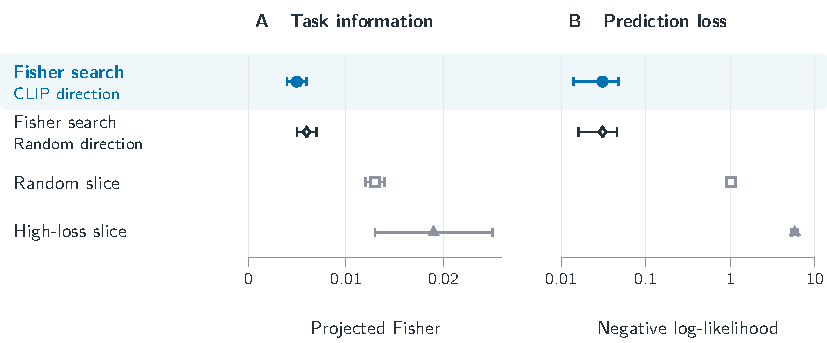
\includegraphics[width=\linewidth]{figures/fig03_discovery.pdf}
\caption[Discovery finds accurate populations with low predictive information]{\textbf{Discovery finds accurate slices with low projected predictive information.}
(A) CLIP-guided search finds low projected predictive Fisher information and 98.8\% membership-weighted accuracy; the random-direction control also attains low information. (B) Both searches yield low uncalibrated NLL (log scale). Selectors target 10\% within-class mass. Points show means and bars 95\% Student-$t$ intervals across five paired seeds, with gates frozen before testing.
}
\label{fig:discovery}
\end{figure}
